\documentclass[11pt,a4paper]{report}

% --- Pacchetti Fondamentali ---
\usepackage[utf8]{inputenc}
\usepackage[T1]{fontenc}
\usepackage{lmodern}
\usepackage[italian]{babel}
\usepackage{etoolbox}
\usepackage[margin=1in]{geometry}
\usepackage{amsmath,amssymb}
\usepackage{xcolor}
\usepackage{listings}
\usepackage{enumitem}
\usepackage{titlesec}
\usepackage{fancyhdr}
\usepackage{graphicx}
\usepackage{hyperref}
\usepackage{cleveref}
\usepackage{subfigure}

\crefformat{section}{\S#2#1#3}
\crefformat{subsection}{\S#2#1#3}
\crefformat{subsubsection}{\S#2#1#3}
\crefformat{figure}{#2Figura~#1#3}
\crefformat{footnote}{#2\footnotemark[#1]#3}
\crefformat{table}{#2Tabella~#1#3}

% --- Configurazione Header e Footer ---
\pagestyle{fancy}
\fancyhf{}
\fancyhead[L]{\small Sistemi Operativi Real-Time}
\fancyhead[R]{\small Giuseppe Capasso}
\fancyfoot[C]{\thepage}
\renewcommand{\headrulewidth}{0.4pt}
\usepackage{tikz}
\usetikzlibrary{arrows.meta, positioning, shapes.geometric, decorations.pathreplacing}

% --- Configurazione Colori e Link ---
\definecolor{primary}{RGB}{38, 66, 139} % Blu scuro istituzionale
\definecolor{codebg}{RGB}{245, 245, 245}

\hypersetup{
    colorlinks=true,
    linkcolor=primary,
    urlcolor=primary,
    citecolor=primary,
}

% --- Configurazione Formattazione Codice ---
\lstset{
    backgroundcolor=\color{codebg},
    basicstyle=\ttfamily\small,
    breaklines=true,
    frame=single,
    rulecolor=\color{lightgray},
    captionpos=b,
    xleftmargin=1em,
    xrightmargin=1em
}

% --- Formattazione Titoli ---
\titleformat{\chapter}[display]
  {\normalfont\bfseries\color{primary}}{\huge Capitolo \thechapter}{1ex}{\Huge}
\titlespacing*{\chapter}{0pt}{-20pt}{40pt}

\begin{document}

% --- Frontespizio ---
\begin{titlepage}
    \centering
    \vspace*{4cm}
    {\Huge \textbf{\color{primary} Sistemi Operativi Real-Time}} \\[1.5cm]
    {\Large \textbf{Dispense del Corso}} \\[0.5cm]
    {\large Docente: Giuseppe Capasso} \\[1.5cm]
    {\normalsize \textbf{Cloud Native Development \& Cybersecurity Specialist}} \\
    {\normalsize Istituto Tecnico Superiore (ITS)} \\
    \vfill
    {\normalsize Anno Accademico 2025/2026}
\end{titlepage}

\tableofcontents
\newpage

\chapter{RTOS}

I \textbf{sistemi operativi real-time} (RTOS) sono una classe speciale di sistemi operativi progettati per garantire che le operazioni vengano eseguite entro vincoli di tempo rigorosi. Nei sistemi real-time, oltre alla correttezza del risultato, è essenziale che l'esecuzione avvenga entro un tempo predefinito. Questo vincolo temporale rappresenta la caratteristica distintiva dei sistemi real-time, dove il tempo è un parametro cruciale quanto l'accuratezza del calcolo.

Un sistema in tempo reale ha un doppio criterio di correttezza:
\begin{itemize}
    \item \textbf{Logico}: il sistema funziona
    \item \textbf{Temporale}: i risultati sono prodotti entro un tempo utile
\end{itemize}

Il criterio temporale è affiancato dalla parola reale in quanto il riferimento temporale deve essere uguale a quello in cui si verificano gli input. Ovvero il tempo interno al sistema deve essere uguale al tempo esterno.

Le principali applicazioni vanno da sistemi multimediali (basate sulla QoS) ai sistemi di controllo di radiazioni, stabilizzatori di volo (Safety critical). I sistemi real-time sono molto usati nei controllori e nei sistemi di controllo digitale.

\begin{figure}[htbp]
    \centering
    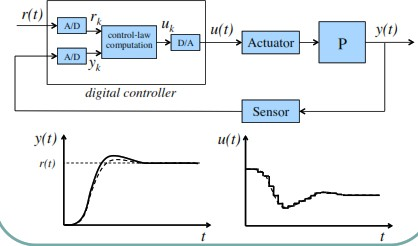
\includegraphics[width=0.6\textwidth]{media/image1.jpeg}
    \caption{Schema di un sistema di controllo digitale}
\end{figure}

Il vantaggio nell'uso di sistemi digitali sta nel fatto che possiamo far eseguire calcoli ad un computer e quindi applicare lo schema di controllo automatizzato. Sorge però un problema: come scegliere il periodo di campionamento e garantire che hardware (CPU e memoria) e software siano in grado di rispettare la deadline?

Il concetto di real-time è completamente diverso da quello di velocità. Quest'ultimo è indicativo delle performance e di valori medi, ma un sistema real-time deve eseguire dei task in maniera indipendente dalla potenza fisica. Il sistema deve essere comunque correttamente dimensionato.

Uno dei primi problemi è la gestione della CPU. Tutti i sistemi eseguono l'astrazione del processo. Questo concetto consente alla CPU di fare più task che possono essere di diverso tipo e non real-time.

Esiste la distinzione tra sistemi (o task):
\begin{itemize}
    \item \textbf{Hard real-time}: il non rispettare la deadline di un processo si possono avere conseguenze catastrofiche.
    \item \textbf{Soft real-time}: non rispettare la deadline porta ad una degradazione della qualità del servizio.
\end{itemize}

Un sistema real-time deve essere \textbf{prevedibile.} Il sistema deve poter consentire di determinare in anticipo tutti i task potranno essere completati entro la propria deadline.

\section{Elementi Base dei Sistemi Operativi Real-Time}

I sistemi operativi real-time si basano su una serie di elementi chiave che garantiscono la gestione efficace delle operazioni entro i vincoli temporali richiesti. Tra questi elementi, i più rilevanti sono:

\begin{itemize}
    \item \textbf{Scheduling dei Processi}: Nei sistemi real-time, lo scheduling deve garantire che i processi critici vengano eseguiti entro scadenze precise. Gli algoritmi di scheduling più comuni includono il \textbf{Rate Monotonic Scheduling (RMS)} per sistemi a priorità statica e lo \textbf{Earliest Deadline First (EDF)} per sistemi a priorità dinamica. Questi algoritmi sono progettati per assicurare che i task più urgenti ricevano la priorità necessaria, minimizzando il rischio di violare i vincoli temporali.

    \item \textbf{Protocolli di Accesso alle Risorse}: La gestione dell'accesso concorrente alle risorse condivise è cruciale nei sistemi real-time. Il \textbf{Priority Inheritance Protocol} e il \textbf{Priority Ceiling Protocol} sono due tecniche utilizzate per prevenire il problema dell'inversione delle priorità, dove un processo a bassa priorità può bloccare un processo più urgente, causando ritardi non accettabili.

    \item \textbf{Gestione delle Interruzioni}: Nei sistemi real-time, le interruzioni devono essere gestite in modo da minimizzare la latenza e garantire che i processi possano reagire rapidamente a eventi esterni. Le interruzioni sono generalmente gestite con priorità molto alta, e i sistemi devono essere progettati per evitare che un'eccessiva frequenza di interruzioni possa compromettere il rispetto delle scadenze temporali.

    \item \textbf{Gestione della Memoria}: La gestione della memoria in un sistema real-time deve essere prevedibile e priva di operazioni che possano introdurre non determinismo, come la paginazione o la sostituzione di pagine. L'uso di memoria statica o di tecniche di allocazione a tempo fisso è comune per ridurre l'incertezza nei tempi di accesso.
\end{itemize}

Questi elementi costituiscono la base della progettazione e implementazione dei sistemi operativi real-time, garantendo che le operazioni critiche possano essere eseguite in modo tempestivo e affidabile.

\subsection{Sfide Attuali nei Sistemi Real-Time}

Attualmente, i sistemi real-time affrontano diverse sfide:
\begin{itemize}
    \item \textbf{Virtualizzazione e Containerizzazione}: Queste tecnologie, sebbene ampiamente adottate per la loro flessibilità, introducono ulteriori livelli di astrazione che possono complicare il rispetto dei vincoli temporali stringenti richiesti dai sistemi real-time.
    \item \textbf{Scalabilità e Parallelismo}: Gestire applicazioni real-time su piattaforme multi-core richiede strategie per minimizzare l'interferenza tra core.
    \item \textbf{Affidabilità e Sicurezza}: L'integrazione di funzioni di sicurezza nei sistemi real-time senza compromettere i vincoli temporali è una sfida continua.
\end{itemize}

\subsection{Tipi di Sistemi Real-Time}

I sistemi real-time si suddividono in diverse categorie a seconda del livello di criticità:
\begin{itemize}
    \item \textbf{Mission-Critical}: Sistemi che devono operare correttamente per garantire il successo di una missione o di un'operazione (ad es. controllo del volo).
    \item \textbf{Safety-Critical}: Sistemi dove un errore potrebbe causare danni a persone, proprietà o all'ambiente (ad es. dispositivi medici, sistemi di controllo industriale).
    \item \textbf{Hard Real-Time}: Sistemi in cui il mancato rispetto delle scadenze temporali può portare a risultati catastrofici.
    \item \textbf{Soft Real-Time}: Sistemi in cui il mancato rispetto delle scadenze non è disastroso, ma potrebbe ridurre la qualità del servizio.
\end{itemize}

\subsection{Predicibilità e Fonti di Non Determinismo}

La \textbf{predicibilità} è un aspetto fondamentale nei sistemi real-time. Affinché un sistema possa essere considerato real-time, deve essere possibile prevedere con certezza i tempi di esecuzione delle operazioni critiche. Tuttavia, diversi elementi hardware e software possono introdurre \textbf{non determinismo}, rendendo difficile garantire il rispetto dei vincoli temporali. Le principali fonti di non determinismo includono:

\begin{itemize}
    \item \textbf{Cache}: Le politiche di gestione della cache (ad es. cache miss) possono introdurre variazioni imprevedibili nei tempi di accesso alla memoria.
    \item \textbf{Architetture Multi-Core}: La concorrenza tra core può causare interferenze nel tempo di esecuzione, soprattutto quando si condividono risorse comuni.
    \item \textbf{Gestione delle Interruzioni}: Le interruzioni hardware e software possono causare ritardi inattesi.
    \item \textbf{Comunicazione Interprocesso}: La sincronizzazione tra processi o thread può introdurre latenze impreviste.
\end{itemize}

I processori moderni seguono delle euristiche per aumentare l'efficienza, ciò li rende imprevedibili (introduce un'incertezza) in quanto lo stesso codice può avere diversi tempi dell'esecuzione (esecuzione pipeline, meccanismi di caching).

L'uso delle \textbf{interruzioni} introduce un concetto asincrono nell'esecuzione del processo che lo rende non più predicibile. In un sistema real-time, le interruzioni sono disabilitate e la comunicazione con le periferiche avviene attraverso:
\begin{itemize}
    \item \textbf{Polling applicativo}: ogni processo esegue delle richieste continue al controller della periferica. I processi diventano più complicati perché devono conoscere il controllore della periferica.
    \item \textbf{Processo di gestione}: un solo processo si occupa di comunicare con il controllore della periferica, mentre i processi real-time comunicano con il gestore (i task real-time sono più semplici).
    \item \textbf{Driver minimale}: viene usato un driver particolare molto semplice che comunica con un processo gestore. La semplicità del driver consente di avere comunque un comportamento deterministico.
\end{itemize}

L'uso delle \textbf{cache} rende un sistema non più predicibile, poiché esiste comunque una probabilità che ci sia una cache miss. Il problema si risolve:
\begin{itemize}
    \item Disabilitando le cache.
    \item Tenendo conto di un fattore moltiplicativo sui tempi di accesso in memoria.
    \item Considerando almeno una cache miss per ogni accesso in memoria. È la tecnica del \textbf{WCET (Worst Case Execution Time)}.
    \item Usando un modello matematico per stimare il numero di cache miss per ogni processo.
\end{itemize}

Le \textbf{system call} di un SO possono essere causa di imprevedibilità a seconda di come sono implementate internamente. In un RTOS le system call devono essere interrompibili anche con le interruzioni disabilitate e devono essere caratterizzate da una durata massima di esecuzione. Ciò consente, in fase di progettazione, di fare delle analisi di schedulabilità ed effettuare il WCET.

Ancora dal punto di vista software, i \textbf{semafori} (responsabili della sincronizzazione tra processi) possono portare ad impredicibilità dovuta alla dipendenza della velocità relativa d'esecuzione dei processi e al noto problema di \textbf{priority inversion}: task ad alta priorità bloccati da task a bassa priorità. L'accesso alle sezioni critiche viene quindi gestito attraverso dei protocolli particolari come:
\begin{itemize}
    \item \textbf{Priority Inheritance}
    \item \textbf{Priority Ceiling}
    \item \textbf{Stack Resource Policy}
\end{itemize}

Altro problema è quello della gestione della memoria. Si preferisce utilizzare un meccanismo di partizionamento statico o dinamico in quanto consente una predicibilità alta. In generale, \textbf{pre-allocare le risorse per un processo rende la sua esecuzione predicibile, ma il sistema poco flessibile.} In un RTOS, è sconsigliato usare la memoria virtuale in quanto introduce altri elementi di impredicibilità quali:
\begin{itemize}
    \item Caching della MMU
    \item Pagefault
    \item Algoritmi di sostituzione delle pagine
\end{itemize}

\subsection{Applicazioni Principali}

I sistemi real-time sono impiegati in una vasta gamma di settori, tra cui:
\begin{itemize}
    \item \textbf{Industria}: Controllo di processi industriali, robotica avanzata, automazione.
    \item \textbf{Aerospazio e Difesa}: Sistemi di guida e navigazione, controllo del traffico aereo.
    \item \textbf{Sanità}: Dispositivi medici, sistemi di monitoraggio dei pazienti.
    \item \textbf{Automotive}: Sistemi di assistenza alla guida (ADAS), controllo del motore.
\end{itemize}

\section{Tipologie di sistemi real-time}

Per capire come implementare sistemi real-time, bisogna cercare di avere una stima corretta della latenza dei task. Questo fenomeno può essere modellato come il tempo che effettivamente intercorre tra l'istante di rilascio $t$ e quello di inizio esecuzione $t'$. Infatti,
\[ L = t' - t \]
ed è possibile dividerlo in 3 componenti:

\begin{figure}[htbp]
    \centering
    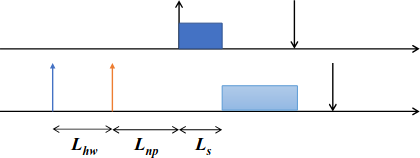
\includegraphics[width=0.5\textwidth]{media/image3.png}
    \caption{Componenti della latenza}
\end{figure}

\begin{itemize}
    \item $L_{hw}$: latenza hardware. Si tratta del ritardo generato dall'interruzione fisica. Di solito questo valore risulta trascurabile ed è esclusivamente dato dalle specifiche tecnologiche della piattaforma. Può essere non trascurabile se si utilizzano timer a bassa risoluzione.
    \item $L_{np}$: sezioni non preemptive della ISR e delle system call. Di solito sono implementati con spinlock e sono richiesti perché il kernel durante un'interruzione deve aggiornare risorse critiche.
    \item $L_s$: latenza data dallo scheduling. Principalmente è data dall'algoritmo specifico e dall'interferenza dei task a priorità più alta. Viene trattata a parte nei test di schedulabilità.
\end{itemize}

\subsection{Real-time executives}

In questo tipo di architettura, i task real-time sono direttamente collegati al sistema operativo e non c'è distinzione tra user mode e kernel mode.

\begin{figure}[htbp]
    \centering
    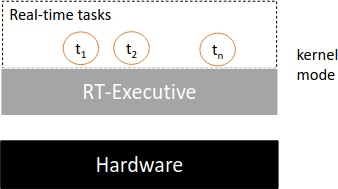
\includegraphics[width=0.4\textwidth]{media/image4.png}
    \caption{Architettura Real-time Executive}
\end{figure}

In applicazioni semplici, la dimensione dell'eseguibile è molto piccola.
 Anche se si tratta di un approccio semplice ha molti svantaggi:
\begin{itemize}
    \item Il codice applicativo interagisce con l'hardware.
    \item Il codice applicativo esegue codice privilegiato.
    \item Il codice applicativo può disabilitare le interruzioni per un intervallo di tempo arbitrario.
\end{itemize}
Questo rende i task applicativi e il sistema operativo strettamente accoppiati. Il massimo $L_{np}$ dipende dal tempo massimo con cui un task tiene le interruzioni bloccate.

\subsection{Kernel monolitici}

Si parla di sistemi operativi Unix-like che separano task utente e task kernel. Possono essere di due tipi:
\begin{itemize}
    \item \textbf{Single threaded}: un solo flusso esecutivo che semplifica la gestione delle risorse. È anche detto \textbf{non-preemptable kernel}: la sincronizzazione delle risorse critiche viene fatta o con la disabilitazione delle interrupt o con un grande kernel-lock. $L_{np}$ è limitato dalla system call che blocca le interruzioni più a lungo possibile.
    \item \textbf{Multi-threaded}: rimuovono i lock globali e usano controlli più fini. Per le sezioni critiche si utilizza \textbf{NPP}. Infatti, un task non real-time che usa una system call può provocare un deadline miss di un task real-time.
\end{itemize}

\subsection{Highest Locking Priority in real-time kernels}

Uno dei protocolli più efficaci è Highest Locking Priority\footnote{\url{https://retis.santannapisa.it/luca/AdvancedOS/Old-22/Slides/resource_sharing_recap.pdf}}, ma ha bisogno di conoscere in anticipo le risorse richieste dai task. L'idea principale è quella di dividere i task real-time da quelli normali e ciò può essere fatto attraverso due strade:
\begin{itemize}
    \item $\mu$-kernel
    \item Dual kernels
\end{itemize}

\subsubsection{$\mu$-kernel}

Un $\mu$-kernel implementa funzionalità utente standard con task server. I task real-time sono implementati come task nativi che eseguono sul kernel e hanno priorità maggiore rispetto ai server utente.

\begin{figure}[htbp]
    \centering
    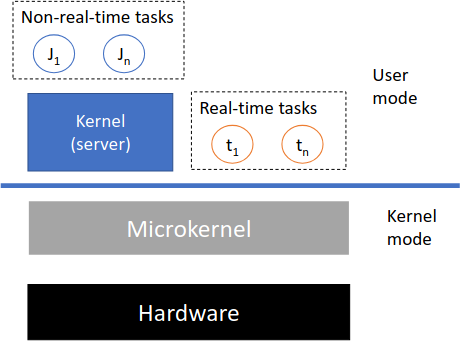
\includegraphics[width=0.5\textwidth]{media/image5.png}
    \caption{Architettura Microkernel}
\end{figure}

Il micro-kernel è composto solo da funzionalità principali che permettono l'IPC, lo scheduling e la gestione della memoria.

Il microkernel deve rimanere abbastanza piccolo da essere non-preemptable e stare tutto nella memoria cache. Le system call e le ISR devono essere il più brevi possibile in modo tale che la latenza di un micro-kernel deve essere sempre inferiore a quella di un kernel monolitico.

Le implementazioni più famose sono quelle della famiglia L4 che hanno dimostrato di essere molto più efficienti dei kernel monolitici con IPC molto più efficienti delle soluzioni dell'epoca. Il principio fondamentale della famiglia L4 è:
\begin{quote}
    Un'entità è considerata accettata all'interno del micro-kernel solo se spostandola all'interno del kernel verrebbe impedita l'implementazione di una funzionalità di sistema.
\end{quote}

\chapter{RTOS-Scheduling}

Nei sistemi real-time, i task hanno \textbf{vincoli temporali} e pertanto bisogna dimostrare (e garantire) che dato un task set sia possibile effettuare una \textbf{schedulazione feasible}. Alcuni indici utilizzati per valutare le prestazioni di un algoritmo sono:

\begin{itemize}
    \item \textbf{Fattore di utilizzazione}: $U = \sum \frac{C_i}{T_i}$
    \item \textbf{Fattore di densità}: $dens = \sum \frac{C_i}{\min(D_i, T_i)}$
\end{itemize}

Una schedulazione è \textbf{feasible} se e solo se tutti i task completano entro la loro deadline.

\section{Modelli di task}

Per i sistemi real-time esistono due modelli utilizzati per esprimere al meglio i vincoli temporali di un problema di scheduling.

\subsection{Modello di Liu e Layland}

In questo modello, un task $\tau_i$ è caratterizzato da $C_i$ (\textbf{Worst case execution time (WCET)}) e da $T_i$ (periodo o tempo di inter-arrivo). Il primo job può arrivare in qualsiasi istante e due istanze successive sono separate da $T_i$. Un sistema di task di Liu e Layland è composto da un insieme finito di task $\{\tau_1, \ldots, \tau_n\}$ che esegue su una piattaforma condivisa. Un task può potenzialmente generare un numero infinito di job.

\subsection{Modello sporadico a tre parametri}

Questo particolare modello prevede l'aggiunta di una deadline relativa $D_i$ in aggiunta a $C_i$ e $T_i$. Quindi $\tau_i = (C_i, D_i, T_i)$. Deadline relativa e periodi possono avere delle relazioni:
\begin{itemize}
    \item \textbf{Deadline implicita}: $D_i = T_i$. Coincide con il modello di Liu e Layland.
    \item \textbf{Deadline vincolata}: $D_i \le T_i$.
    \item \textbf{Deadline arbitraria}: Non ci sono relazioni tra deadline e periodi.
\end{itemize}

\section{Scheduling a priorità}

Nella comunità real-time, sono molto utilizzati gli scheduler a priorità. Una prima classificazione:
\begin{itemize}
    \item \textbf{Fixed task priority (FTP)}: ai task $\tau_i$ viene assegnata una priorità fissa $P_i$ e questa viene ereditata da tutti i job $J_i$ generati da $\tau_i$. Un algoritmo FTP è \textbf{Rate monotonic}.
    \item \textbf{Fixed job priority (FJP)}: a job differenti dello stesso task $\tau_i$ viene assegnata una priorità diversa in base alla situazione corrente. Un algoritmo FJP è \textbf{Earliest Deadline First}.
    \item \textbf{Dynamic priority (DP)}: la priorità di un job può essere assegnata in maniera dinamica. Un algoritmo DP è il \textbf{pfair}.
\end{itemize}

\section{Scheduling di task aperiodici}

Un task aperiodico $J_i$ è il tipo di task più semplice. Possono arrivare tutti allo stesso momento ($a_i = 0$) o con ordine sparso.

\textbf{Algoritmo di Jackson ($1|sync|L_{max}$)}
Assume che tutti i task arrivano allo stesso momento e per ciascuno sono noti $D_i$ e $C_i$. I task sono indipendenti. L'algoritmo ordina i task per deadline in ordine non decrescente (\textbf{Earliest Due Date}). Minimizza la massima lateness $L_{max}$. Lavora in $O(n \log n)$ ed è ottimo.

\textbf{Algoritmo di Horn ($1|preem|L_{max}$)}
Rimuove l'ipotesi di arrivo sincrono. È indispensabile la preemption. Esegue il task con deadline assoluta più vicina. È una versione dinamica di EDD. Fornisce una schedulazione ottima. Essendo online, è necessario eseguire un test di schedulabilità ad ogni attivazione:
\[ \forall i = 1 \ldots n \quad \sum_{k=1}^{i} c_k(t) \le d_i \]
L'algoritmo è detto \textbf{Earliest Deadline First (EDF)}.

\subsection{Non preemptive-scheduling}

Quando non è consentita la prelazione, il problema dello scheduling con ipotesi di arrivo non sincrono diventa non trattabile. Questo tipo di problemi può essere risolto con diversi approcci. Una soluzione può essere adottare algoritmi che permetta al processore di essere in idle. Altri algoritmi possono essere trattati con branch and bound ed esplorazione di alberi che sfociano in complessità esponenziali. Inoltre, queste tecniche non assicurazioni soluzioni ottime, ma semplicemente fattibili.

\begin{figure}[htbp]
    \centering
    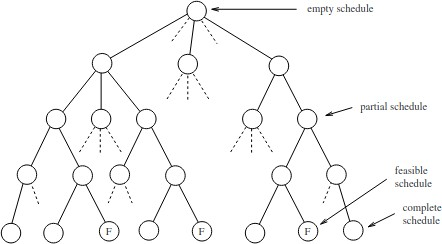
\includegraphics[width=0.5\textwidth]{media/image6.jpeg}
    \caption{Esempio di esplorazione ad albero per scheduling non preemptive}
\end{figure}

\section{Scheduling di task periodici}

In un sistema real-time, la maggior parte del lavoro è svolto da task periodici.

\subsection{Modello di task}

Ogni istanza $j$ del task $i$ è caratterizzata da:
\begin{itemize}
    \item Tempo di arrivo $a_{i,j}$ (o release time $r_{i,j}$)
    \item Tempo di inizio esecuzione $s_{i,j}$
    \item Tempo di fine esecuzione $f_{i,j}$
    \item Prima esecuzione $\Phi_i = r_{i,1}$
    \item Deadline relativa $D_i$
    \item Tempo di calcolo $C_i = f_{i,j} - s_{i,j}$
    \item Deadline assoluta $d_{i,j} = \Phi_i + (j-1)T_i + D_i$
\end{itemize}

Parametri del task set:
\begin{itemize}
    \item Iperperiodo $H = mcm(T_1, \ldots, T_n)$
    \item Utilizzazione del processore $U = \sum_{i=1}^{n} \frac{C_i}{T_i}$
\end{itemize}

\subsection{Timeline scheduling}

Algoritmo più semplice. L'asse dei tempi è partizionata in slot di uguali dimensioni (\textbf{minor cycle}) gestiti con un timer (la durata del singolo slotè l'$MCD$ tra il periodo dei task).

\begin{figure}[htbp]
    \centering
    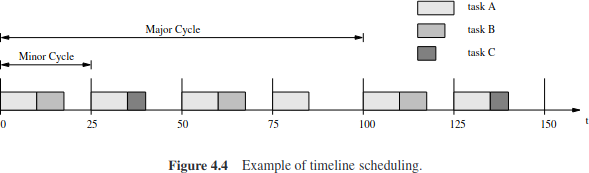
\includegraphics[width=0.7\textwidth]{media/image7.png}
    \caption{Timeline Scheduling}
    \label{fig:timeline-scheduling-ex}
\end{figure}

L'iperperiodo è il \textbf{major cycle} (calcolato come l'$mcm$ tra i periodi dei task). Il test di schedulabilità verifica che in ogni slot la somma dei tempi di esecuzione non superi il minor cycle. Ad esempio, in \cref{fig:timeline-scheduling-ex}, $T_A=25ms, T_B=50ms, T_C=100ms$. Il minor-cycle è $25ms$ e il test diventa:

\begin{equation}
    \begin{cases}
        C_A + C_B \leq 25ms\\
        C_A + C_C \leq 25ms\\
    \end{cases}
\end{equation}

\subsection{Rate Monotonic (RM)}

Algoritmo a priorità fissa che assegna priorità crescente in base alla frequenza di un task. Un task ad alta frequenza avrà priorità maggiore. L'algoritmo richiede la prelazione in quanto un task deve essere sospeso se ne arriva uno nuovo con periodo inferiore. L'algoritmo assume che la deadline relativa di un task coincida con il suo periodo.

Liu e Layland hanno dimostrato che Rate Monotonic è ottimo tra tutti gli algoritmi a priorità fissa e hanno anche fornito una condizione sufficiente per capire se un dato task set è schedulabile:
\[ \sum_{i=1}^{n} \frac{C_i}{T_i} \le n(2^{1/n} - 1) \]

\begin{figure}[htbp]
    \centering
    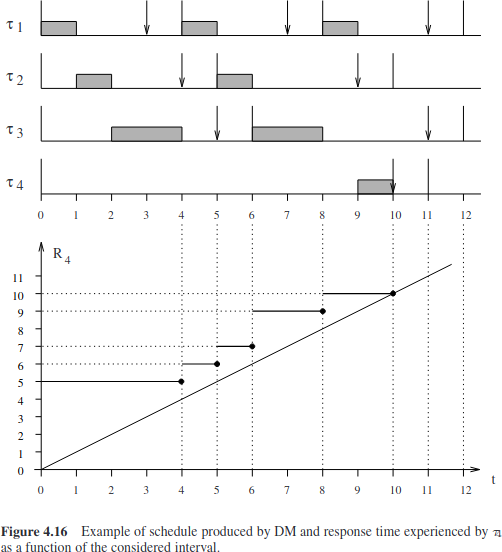
\includegraphics[width=0.6\textwidth]{media/image11.png}
    \caption{Esempio di scheduling Rate Monotonic}
\end{figure}

\textbf{Response Time Analysis (RTA)}

Il test di Liu e Layland risulta pessimistico. Infatti, è un upper bound e può essere migliorato con un'analisi più fine detta RTA (Response Time Analysis). La RTA consiste nel calcolare il tempo di esecuzione di un task includendo, oltre al suo $C_i$, anche il tempo di calcolo dei task a priorità più alta che potrebbero interrompere il task causando un'interferenza.

Supponendo di aver ordinato i task per priorità così che $p_i > p_j$ se $i < j \leftrightarrow D_i < D_j$. L'interferenza del task $i$ è data dalla somma dei tempi di calcolo $C_k$ di tutti i task $\tau_k$ con $0 < k < i$ (ovvero quelli a maggiore priorità di $i$) per il numero di volte in cui questo interrompe il task $\tau_k$. Quindi:
\[ I_i = \sum_{k=1}^{i-1} \left\lceil \frac{R_i}{T_k} \right\rceil C_k \]

Quindi $R_i = C_i + I_i$, sostituendo si ottiene:
\[ R_i = C_i + \sum_{k=1}^{i-1} \left\lceil \frac{R_i}{T_k} \right\rceil C_k \]

Come si vede dalla formula l'interferenza non può essere calcolata in forma chiusa, ma in forma iterativa. Intuitivamente, il test di schedulabilità si riduce a:
\[ \forall i = 1 \ldots n \quad R_i \le D_i \]
La ricorrenza viene risolta ponendo $R_i^{(0)} = \sum_{k=1}^{i} C_k$:
\[ R_i^{(s)} = C_i + \sum_{k=1}^{i-1} \left\lceil \frac{R_i^{(s-1)}}{T_k} \right\rceil C_k \]

\textbf{Esempio di RTA iterativa:}
Si consideri un task set dove bisogna calcolare il response time di $\tau_4$.
L'interferenza di $\tau_4$ è: $I_4^k = \sum_{j=1}^{3} \lceil \frac{R_4^k}{T_j} \rceil C_j$.

Sotto sono riportate le 4 iterazioni:
\begin{itemize}
    \item \textbf{Step 0}: $R_4^{(0)} = \sum_{i=1}^{4} C_i = 5$, but $I_4^{(0)} = 5$ and $I_4^{(0)} + C_4 > R_4^{(0)}$ hence $\tau_4$ does not finish at $R_4^{(0)}$.
    \item \textbf{Step 1}: $R_4^{(1)} = I_4^{(0)} + C_4 = 6$, but $I_4^{(1)} = 6$ and $I_4^{(1)} + C_4 > R_4^{(1)}$ hence $\tau_4$ does not finish at $R_4^{(1)}$.
    \item \textbf{Step 2}: $R_4^{(2)} = I_4^{(1)} + C_4 = 7$, but $I_4^{(2)} = 8$ and $I_4^{(2)} + C_4 > R_4^{(2)}$ hence $\tau_4$ does not finish at $R_4^{(2)}$.
    \item \textbf{Step 3}: $R_4^{(3)} = I_4^{(2)} + C_4 = 9$, but $I_4^{(3)} = 9$ and $I_4^{(3)} + C_4 > R_4^{(3)}$ hence $\tau_4$ does not finish at $R_4^{(3)}$.
    \item \textbf{Step 4}: $R_4^{(4)} = I_4^{(3)} + C_4 = 10$, but $I_4^{(4)} = 9$ and $I_4^{(4)} + C_4 = R_4^{(4)}$ hence $\tau_4$ finishes at $R_4 = R_4^{(4)} = 10$.
\end{itemize}

\begin{figure}[htbp]
    \centering
    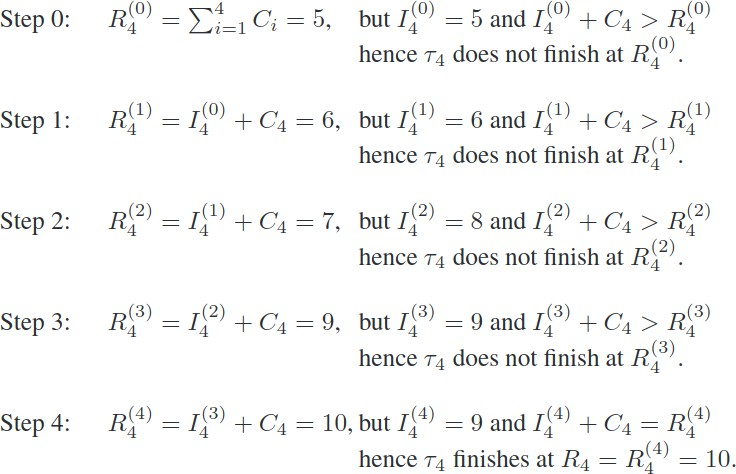
\includegraphics[width=0.6\textwidth]{media/image12.jpeg}
    \caption{Rappresentazione grafica delle iterazioni RTA}
\end{figure}

\subsection{Deadline Monotonic (DM)}

Variante di RM per $D_i < T_i$. Priorità in base alla deadline relativa: deadline minore $\to$ priorità maggiore.

\subsection{Earliest Deadline First (EDF)}

Algoritmo dinamico: esegue il task con deadline assoluta più vicina. Ottimo. Test di schedulabilità:

\begin{equation}
U \leq 1 \to \sum_{i=1}^n\frac{C_i}{T_i} \leq 1
\end{equation}

\section{Server aperiodici}

Gli algoritmi analizzati fino ad ora assumono che i task set siano omogenei (solo task aperiodici o solo task periodici). Nella realtà, il workload di un sistema real-time è formato sia da task periodici (time driven: sensori, loop di controllo ecc.) che task aperiodici (event driven). In generale, si assume che i task periodici siano real-time, mentre quelli aperiodici non sono critici, ma debbano avere una certa QoS.

I processi aperiodici possono essere sporadici se è garantito un intervallo di tempo minimo tra due occorrenze:
\[ a_{i,k+1} > a_{i,k} + \delta_i \]

L'approccio utilizzato è quello di schedulare la parte periodica con uno degli algoritmi visti in precedenza (EDF, RM o DM) e di usare un processo (\textbf{server aperiodico}) per la gestione del carico aperiodico. In generale, il server aperiodico è dotato di:
\begin{itemize}
    \item \textbf{Banda} $C_s$: tempo di calcolo con cui servire i task aperiodici.
    \item \textbf{Periodo} $T_s$ di esecuzione.
\end{itemize}

I server aperiodici sono distinti in processi a priorità fissa e dinamica. È possibile evitare l'utilizzo di un server schedulando il carico aperiodico in background.

\subsection{Background scheduling}

Se i task aperiodici non sono real-time, si possono eseguire in background: quando non c'è carico periodico. Questo approccio è molto semplice da implementare: la coda dei task aperiodici viene servita solo se quella periodica è vuota. L'arrivo di un task periodico causa preemption sul processo aperiodico.

\begin{figure}[htbp]
    \centering
    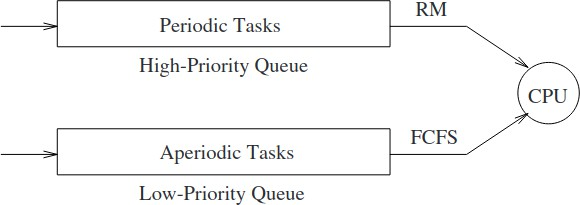
\includegraphics[width=0.7\textwidth]{media/image15.jpeg}
    \caption{Esempio di Background Scheduling}
\end{figure}

Svantaggio: lunghi tempi di risposta per i processi aperiodici se il carico periodico è molto alto.

\subsection{Polling server (PS)}

Caratterizzato da $C_s$ e $T_s$, viene trattato come un processo periodico e schedulato (es. con RM). Quando viene schedulato, il server verifica se esistono richieste aperiodiche. Se sì, le esegue fino a esaurimento di $C_s$. Il budget si ricarica ad ogni periodo. Se non trova task, si sospende fino alla prossima attivazione.

\begin{figure}[htbp]
    \centering
    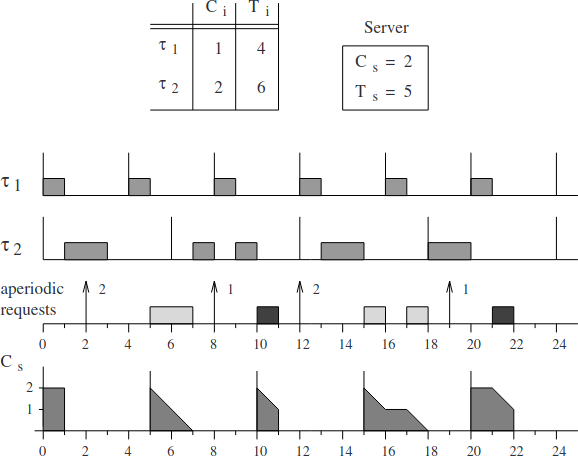
\includegraphics[width=0.6\textwidth]{media/image17.png}
    \caption{Esempio di Polling Server}
\end{figure}

Test di schedulabilità (estensione di Liu e Layland):
\[ \sum_{i=1}^{n} \frac{C_i}{T_i} + \frac{C_s}{T_s} \le (n+1)(2^{1/(n+1)} - 1) \]

\subsection{Deferrable server (DS)}

Il DS modifica il PS mantenendo la capacità anche quando non ci sono task presenti durante l'attivazione. In questo caso, il DS viene servito come task periodico, ma può usare la sua banda quando ci sono task aperiodici in pending. Terminata, la capacità questa viene riempita ad ogni periodo.

Dal punto di vista della garanzia dello scheduling, il DS non può essere considerato come un processo periodico in quanto non utilizza tutta la sua capacità all'attivazione, ma la conserva causando delle possibili interferenze non presenti con il PS (da qui il nome deferrable -> defers).

\begin{equation}
    U_p \leq n \cdot \big[\big(\frac{U_s + 2}{2U_s + 1})^{1/n} - 1]
\end{equation}

\begin{figure}[htbp]
    \centering
    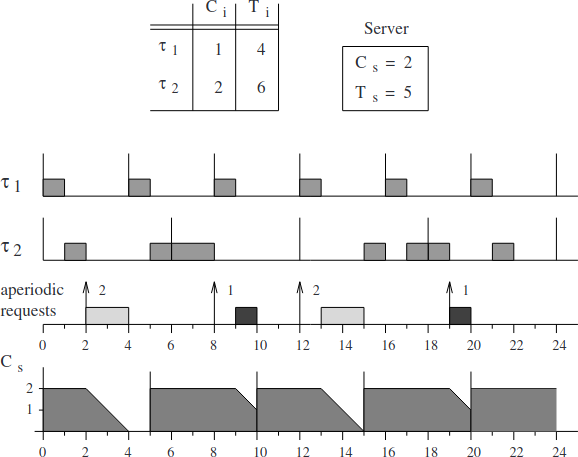
\includegraphics[width=0.6\textwidth]{media/image18.png}
    \caption{Esempio di Deferrable Server}
\end{figure}

\subsection{Sporadic server (SS)}

Migliora il tempo di risposta senza intaccare il carico periodico. La capacità non viene riempita ad ogni periodo, ma solo dopo essere stata consumata. Calcola il \textbf{replenishment time (RT)} e il \textbf{replenishment amount (RA)}.

\begin{figure}[htbp]
    \centering
    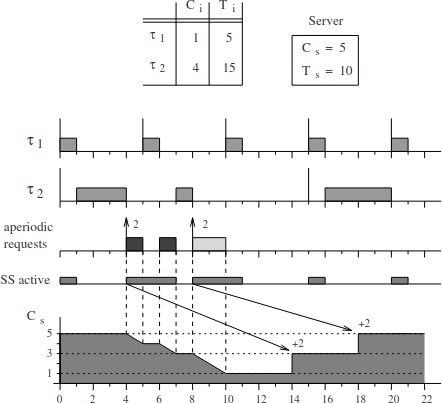
\includegraphics[width=0.5\textwidth]{media/image20.png}
    \caption{Esempio di Sporadic Server}
\end{figure}

$SS$ viene schedulato da $RM$ sulla base del suo periodo $T_s$. [Si dimostra](Sprunt, Sha, Lehoczky) che un insieme di task periodici con un task $\tau_i$ risulta essere ancora schedulabile se $\tau_i$ è rimpiazzato da un Server Sporadico con stesso periodo $T_s$ e tempo di calcolo $C_s$.

Definiti i seguenti termini:
\begin{itemize}
    \item $P_{exe}$ priorità del processo in esecuzione;
    \item $P_S$ priorità del server;
    \item Active: il server è detto active se $P_{exe} \geq P_s$;
    \item Idle: Il server è detto in idle se $P_{exe} \le P_s$;
\end{itemize}

Quando il server diventa attivo e $C_s$ > 0 all'istante $t_A$, allora $RT = t_A + T_S$. Quando il server diventa idle ($t_I$) o viene consumata la capacità, allora RA è pari alla capacità consumata in $[t_A, t_I]$.

\begin{figure}
    \centering
    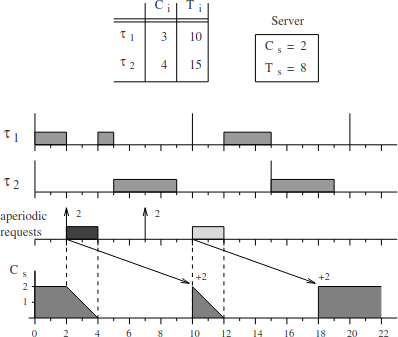
\includegraphics[width=.5\textwidth]{media/image21.png}
    \caption{Esempi di SS a priorità media}
\end{figure}

\subsection{Dynamic Sporadic Server (DSS)}

Versione dinamica di SS utilizzata con EDF. La capacità viene ricaricata in base alla deadline del server. In pratica, SS viene schedulato con RM in base al suo periodo $T_s$. La versione dinamica viene utilizzata con EDF e, pertanto, la sua deadline, RT e RA sono definite con le seguenti regole:

\begin{itemize}
    \item il server viene inizializzato con $C_s$ massima;
    \item $RT = d_s$ appena arriva una richiesta aperiodica e $C_s \ge 0$ in $t_A$ segue che $RT= d_s =  t_A + T_S$;
    \item $RA$ viene calcolata quando viene servita l'ultima richiesta aperiodica o quando $C_s = 0$. Detto $t_I$ questo istante, allora $R_A$ è la quantità di capacità consumata in $[t_A, t_I]$
\end{itemize}

Utilizzando EDF il test di schedulabilità diventa molto semplice. Detto $U_s = \frac{C_s}{T_s}$, e $U_p$ l'utilizzazione del carico periodico, allora un insieme di task periodici con un DSS è schedulabile con EDF se e solo se:

\begin{equation}
    U_S + U_p \leq 1
\end{equation}

\begin{figure}[htbp]
    \centering
    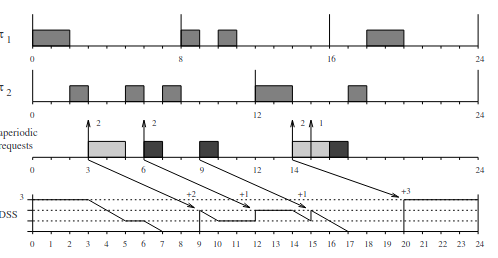
\includegraphics[width=0.6\textwidth]{media/image24.png}
    \caption{Dynamic Sporadic Server}
\end{figure}

Il problema con gli SS è che con periodi lunghi i task aperiodici diventano meno responsivi. Fare periodi corti non conviene perchè poi bisogna abbassare anche la capacità e questo comporta RT frequenti che aumentano il numero di context switch sul carico periodico.

\subsection{Total Bandwidth Server (TBS)}

Il TBS fa parte della classe dinamica dei server aperiodici. In particolare, data una capacità $C_s$ e un periodo $T_s$, il server si occupa di calcolare una deadline per ogni richiesta aperiodica che sarà così schedulata con il carico periodico. In particolare, supposto che $J_k$ arrivi con $r_k$, la sua deadline sarà calcolata dando tutta la banda del server disponibile. Quindi, detto $U_s = \frac{C_s}{T_s}$:
\[ d_k = \max(r_k, d_{k-1}) + \frac{C_k}{U_s} \]

Si dimostra che la condizione di schedulabilità per questo sistema è: $U_s + U_p \le 1$.

\subsection{Constant Bandwidth Server (CBS)}

Fornisce un meccanismo di priorità dinamica (usato con EDF). Caratterizzato da $(Q_s, T_s)$, dove $Q_s$ è la capacità massima; la capacità corrente è $c_s$. La banda è $U_s = Q_s / T_s$. Ogni job aperiodico riceve una deadline dinamica $d_{s,k}$ (con $d_{s,0} = 0$) pari a quella del server. Se il budget $c_s$ si esaurisce, viene ricaricato e la deadline viene posticipata: $d_{s,k+1} = d_{s,k} + T_s$.

Il server funziona con le seguenti regole:
\begin{itemize}
    \item Ogni $J_{i,j}$ ha una deadline dinamica $d_{i, j} = d_{s,k}$ (pari a quella corrente del server);
    \item quando $c_s = =0$ questo viene subito ricaricao a $Q_s$ e viene generata una nuova deadline con $d_{s, k + 1} = d_{s,k} + T_s$;
    \item il CBS è attivo all'istante $t$ quando ci sono job in coda e $c_s \ge 0$ ovvero se esiste un job $J_{i, j}$ tale che $r_{i, j} \leq t \leq f_{i, j}$; altrimenti è in \textbf{idle};
    \item Quando arriva un job e il server è in idle:
        \begin{itemize}
            \item Se $c_s \geq (d_{s,k} - r_{i, j})U_s$ allora il server genera una nuova deadline $d_{s,k+1} = r_{i, j} + T_s$ e pone $c_s = Q_s$
            \item Atrimenti viene servita la richiesta mantenendo la deadline
        \end{itemize}
    \item quando un job termina viene preso il prossimo dalla coda
\end{itemize}

l test di schedulabilità rimane uguale al TBS. Un insieme di $n$ task periodici con $U_p$ e un insieme di $m$ CBS con utilizzazione $U_s = \sum_{i = 1}^m U_{si}$, l'insieme risulta schedulabile se e solo se  $U_s + U_p \le 1$.


\subsection{Hard CBS}

I server aperiodici possono essere divisi in:
\begin{itemize}
    \item \textbf{Hard reservation}: quando termina la capacità, il server si sospende fino alla prossima attivazione (PS, DS, SS, DSS).
    \item \textbf{Soft reservation}: la capacità viene subito riempita quando termina così il server rimane sempre attivo (\textit{backlogged}, TBS, CBS). Soffrono del problema di \textbf{deadline aging}.
\end{itemize}

Una garanzia per la latenza delle richieste aperiodiche può essere ottenuta modificando il CBS classico (Hard CBS) e assumendo che la richiesta $J_i$ abbia $D_i \ge T_s$ e $C_i \le C_s$. Bisogna modificare la regola di allocazione della banda quando arriva un task aperiodico e il server è in idle:
\begin{enumerate}
    \item Si calcola $RT = d_s - \frac{c_s}{U_s}$.
    \item Se $t < RT$ il server si sospende e riprende a $RT$ con $c_s = C_s$ e $d_s = RT + T_s$.
    \item Altrimenti il server non si sospende e $c_s = C_s$ e $d_s = t + T_s$.
\end{enumerate}
Quando il budget termina ($c_s = 0$) il server si sospende fino a $d_s = d_s + T_s$.

\begin{figure}[htbp]
    \centering
    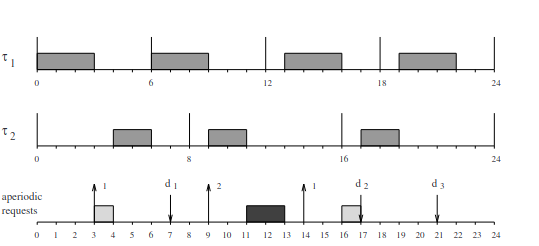
\includegraphics[width=0.6\textwidth]{media/image25.png}
    \caption{Esempio di Hard CBS}
\end{figure}

\section{Multi-core scheduling}

Lo scheduling multi-core prevede 3 modelli di piattaforme:
\begin{itemize}
    \item \textbf{Identici}:  questi sistemi hanno tutti i processori identici ciascuno con le stesse capacità di calcolo degli altri
    \item \textbf{Uniformi}: processori con velocità differenti. Un job esegue su un processore di capacità $s$ per un tempo $t$ completando in $s \cdot t$ unità di lavoro.
    \item \textbf{Unrelated}:  in questo caso ogni processore può avere un rate differente in base al singolo job. Un job che esegue su un processore con rate $r$ per un tempo $t$, completerà la sua esecuzione per $r \cdot t$ unità di tempo;
\end{itemize}

Job diversi di task diversi possono eseguire in maniera simultanea su più core. I modelli che si considerano, fanno in modo tale che per ogni istante un task risulti in esecuzione su un solo processore. Non è previsto il parallelismo all'interno dello stesso job. Gli scheduler multi-core sono divisi in due grandi famiglie:

\begin{itemize}
    \item \textbf{Partizionati}: i job sono assegnati a un core e non migrano.
    \item \textbf{Globali}: i job possono migrare tra core.
\end{itemize}

Quando si parla di multi-core scheduling è necessario estendere la tassonomia del caso single-core. Con la legge di Moore, non si creano più chip single core. È necessario quindi affrontare questo problema. La base di partenza sono i modelli Liu e Layland e quello sporadico a tre parametri.

\subsection{Fixed Partitioned scheduling (con EDF)}

Questo algoritmo si applica ad un task set $\tau$ di Liu e Layland con deadline implicita e un sistema con m processori. I task devono essere partizionati in m sottoinsiemi disgiunti. I task assegnati ad un processore sono schedulati con EDF. Dalla teoria dello scheduling uniprocessore, si dimostra che EDF è ottimo e che una condizione necessaria e sufficiente per la schedulabilità è che
\begin{equation}
    \sum_{i=1}^n \frac{C_i}{T_i} \leq 1
\end{equation}

\subsection{Reasonable allocation}

Un algoritmo RA viene definito come uno che fallisce nell'allocazione di un task su un sistema multiprocessore solo quando l'utilizzazione del task eccede l'utilizzazione residua di tutti i processori.

In generale, un task \textit{fit} su un processore se la sua utilizzazione $\frac{C_i}{T_i}$ non eccede quella del processore $m_j$ esclusa la somma di tutte le capacità dei task già schedulate su di esso. Questo è un problema di \textbf{bin packing} (NP-Completo). Per questo motivo è necessario definire delle euristiche che consentono di scegliere assegnare i task ai
processori:

\begin{itemize}
    \item \textbf{First Fit (FF)}: ): un task viene assegnato sul primo processore che ha abbastanza utilizzazione per poterlo ricevere;
    \item \textbf{Best Fit (BF)}: un task viene assegnato ad un processore con minima utilizzazione rimasta su cui entra il task;
    \item \textbf{Worst Fit (WF)}: un task viene assegnato al processore con la massima utilizzazione rimasta;
\end{itemize}

Inoltre, si definiscono delle euristiche con le quali si prendono i task:
\begin{itemize}
    \item \textit{I}: i task vengono presi in ordine crescente di utilizzazione;
    \item \textit{D}: i task vengono presi in ordine decrescente di utilizzazione;
    \item \textit{$\epsilon$}: i task vengono presi in ordine arbitrario;
\end{itemize}

Quindi, il prodotto cartesiano $\{BF , WF , FF\}x\{I, D, \epsilon\}$ genera 9 combinazioni possibili ciascuno con i propri vantaggi e svantaggi. Le combinazioni sono denotate come BFI, WFD.

\subsubsection{Utilization Bound}
Dato un set di task $\tau$ che deve essere schedulato su $m$ processori, $\alpha$ il massimo utilization bound di un task e $\beta = \lceil \frac{1}{\alpha}\rceil$
si dimostrano i seguenti vincoli.

\paragraph{Minimo utilization bound}
Si può notare che se un task $\tau_i$ (con utilizzazione $u_i$) non può essere schedulato, allora deve essere che ciascun processore ha almeno allocato $(1 - u_i)$. Quindi sommando per ogni processore, si ottiene $m(1 - u_i)$. Da cui si deduce che l'utilizzazione totale non può essere più piccola di $m - (1 - m)\alpha$.
\begin{align}
    m(1-u_i) + ui &= \\
    &= m - m \cdot u_i + u_i \\
    &= m - (1 - m)u_i \\
    &= m - (1 - m)\alpha\; detto \;\alpha \geq u_i
\end{align}

\paragraph{Massimo utilization bound}

Si dimostra che il l'upper bound per l'utilizzazione totale è:

\begin{equation}
    U_b = \frac{\beta m + 1}{\beta + 1}
\end{equation}

\subsection{Variante con RM}
È una variante rispetto a quella con EDF. I task sono assegnati ad un processore a seconda della sua utilizzazione con le euristiche dette in precedenza (FFD, BFI, ecc). A partire dalla schedulazione su singolo processore si trovano i vincoli di least upper-bound. I più famosi sono quelli di \textit{Oh e Baker} e \textit{Diaz e Garcia}. Oh e Baker affermano che un sistema di task sporadici a deadline implicita allocati con euristica FFD su $m$ processori e schedulati con RM è schedulabile se:

\begin{equation}
    U < m (\sqrt{2} - 1)
\end{equation}

Mentre \textit{Diaz, Garcia} offrono una versione più precisa con le stesse ipotesi. Dato un task set $\tau$:

\begin{equation}
    U_{sum}(\tau) < (m-1)(\sqrt{2} - 1) +  (n - m +1)(2^{\frac{1}{n-m+1}} - 1)
\end{equation}


\subsection{Global scheduling}
In questo tipo di scheduling, la migrazione tra processori è consentita. Il teorema di Horn dice che. Un task set $\tau$ è schedulabile su una piattaforma con m processori se:

\begin{equation}
    U_{sum}(\tau) \leq m
\end{equation}

e se:
\begin{equation}
    U_{sum}(\tau) \leq 1
\end{equation}

\subsubsection{Algoritmo pFair}
Algoritmo ottimo per task con deadline implicite in cui ogni job può eseguire su processori differenti in ogni istante. \textbf{pfair} divide il tempo in \textbf{slot} unitari e i job in sotto-job unitari a cui viene assegnata una \textbf{pseudo-deadline}. L'algoritmo pFair si comporta in modo tale che ogni task abbia un progresso proporzionato rispetto agli altri. Questo
fattore è detto fair share all'istante $t$ ed è esattamente:

\begin{equation}
    (t -t_0) u_i
\end{equation}

dove, $t_0$ è l'istante in cui viene rilasciato il task. Inoltre, vale $t_0 \leq t \leq t_0 +T$. Ovvero un task da più tempo è stato rilasciato più avrà un \textbf{fair share} alto. Si dice la schedulazione effettua un \textbf{proportionate progress} se riceve esattamente:

\begin{equation}
    \lceil(t -t_0) u_i\rceil \; oppure \; \lfloor(t -t_0) u_i\rfloor
\end{equation}

Si può dimostrare che che per ogni scheduler che soddisfa il teorema di Horn, esiste una schedulazione pfair. La notazione dell'algoritmo pFair è la seguente:

\begin{itemize}
    \item $\tau$ di task caratterizzati da $C_i$ e $T_i$;
    \item Ogni task $\tau_i$ genera $n_i$ job;
    \item I job vengono rilasciati a $r_{i,k}$ e non sono sovrapponibili $r_{i,k+1}\ge r_{i,k} + T_i$;
    \item $I$ insieme di job generati da $\tau$;
    \item Si assume che $\min_{\tau_i \in \tau}(r_{i,0} = 0)$;
    \item $t_max = \max_{\tau_i\in\tau}(r_{i,n_{i}-1} + T_i)$;
    \item $slot[l]$ indica l'intervallo $[l, l+1)$
\end{itemize}

Si definisce:
\begin{equation}
    alloc(S, \tau_i, t) = \sum_{i\in[0, t] S(x, i)}
\end{equation}

$S$ è una funzione da $\tau x N \to \{0, 1\}$ che definisce per quale slot $t$, $\tau_i$ risulta allocato. In pratica $S(\tau_i, t) = 1$ se $\tau_i$ è schedulato in $\tau$. Quindi deve essere:

\begin{equation}
     \sum_{\tau_i \in \tau} S(\tau_i, t) \leq m
\end{equation}

Si definisce \textbf{lag} rispetto ad $S$, la funzione $lag(S, \tau_i, t)$ che indica la differenza tra quante volte il task dovrebbe essere allocato in $[0, t)$ e quante volte effettivamente lo è stato:

\[ lag(S, \tau_i, t) = \sum_{r_{i,k} \le t} u_i \cdot \min(T_i, (t - r_{i,k})) - alloc(S, \tau_i, t) \]

Una schedulazione è pFair se $\forall \tau_i, t: -1 < lag(S, \tau_i, t) < 1$. Ovvero se per ogni task $\tau_i$ e per ogni $t$ la funzione di lag è strettamente compresa tra $-1$ e $1$.

In generale, tutte queste regole indicano il fatto che la pfairness è un requisito stringente: un task non rimane mai indietro o viene schedulato in anticipo più di uno slot.
Dal punto di vista implementativo pfair è uno scheduler DP ed è chiaro che la suddivisione in slot può portare ad avere tante preemption, context switch e migrazioni che possono condurre a costi non trascurabili.

\subsubsection{Global EDF}
Per gli scheduling globali, EDF è una variante Fixed Job Priority e può essere una soluzione laddove la soluzione Dynamic Priority di pfair non fosse sufficiente a causa dei numerosi context switch, preemption e migrazioni.

Ogni job viene schedulato sul primo processore disponibile seguendo l'ordine delle deadline. Si tratta di una semplice estensione dell'EDF al caso multiprocessore. Tuttavia, la versione multi-core di EDF non è ottima e soffre dell'\textbf{effetto Dhall}.

\paragraph{Global EDF su sistema uniforme}
Un sistema uniforme $\pi$ è formato da $m(\pi)$ processori dove $m(\pi) \in N$. Ogni processore ha la sua capacità di calcolo $\pi = [s_1, s_2, … , s_m(\pi^1)]$ e si ipotizza di ordinarle per potenza: $s_1$ sarà il processore più veloce. Si definiscono gli indici $S_{max}(\pi) = s_1$ e

\begin{equation}
    S_{sum}(\pi) = \sum_{i=1}^{m(\pi')}s_i
\end{equation}

Inoltre, un parametro che denota le differenze dei processori (ovvero quanto il sistema è diverso da uno identico) è:

\begin{equation}
    \lambda(\pi) = \max_{J=1}^{m(s')} \big\{\frac{\sum_{k=j+1}^m(\pi)s_k}{s_j}\big\}
\end{equation}

In pratica, si assume di avere di avere un insieme di job $J_i = (r_i, c_i, d_i)$. Ogni job ha bisogno di eseguire per $c_i$ unità di tempo in $\lceil r_i, d_i)$.

Si assume che EDF è implementato su una piattaforma uniforme se sono soddisfatte le seguenti regole:
\begin{enumerate}
    \item nessun processore viene lasciato in idle quando c'è un job in attesa di essere eseguito;
    \item quando ci sono meno job in attesa che numero di processori, allora viene scelto il processore più veloce mentre quello più lento viene messo in idle;
    \item i processi più prioritari vengono messi in idle. Se un task si trova su un processore $j$, allora quelli che si trovano su $j + 1, j + 2$ ecc hanno una deadline maggiore di quello in esecuzione sul processore $j$;
\end{enumerate}

Le prime due regole formano la definizione di scheduling work conserving.

Un insieme di job I ha una schedulazione fattibile su un sistema uniforme $\pi$, allora una schedulazione EDF di I su un sistema $\pi'$ rispetterà tutte le deadline se è rispettata la seguente condizione su $\pi$ e $\pi'$:

\begin{equation}
    S_{sum}(\pi') \geq \lambda(\pi') \cdot S_{max}(\pi) + S_{sum}(\pi)
\end{equation}

\paragraph{Global EDF su un sistema identico}

Su un sistema identico, un sistema $\pi$ su cui $\tau$ è schedulabile ha le seguenti proprietà:

\begin{enumerate}
    \item $S_{max}(\pi) = U_{max}(\tau)$
    \item $S_{sum}(\pi) = U_{sum}(\tau)$
\end{enumerate}

Il limite di utilizzazione per un insieme $\tau$ con EDF su $m$ processori identici è:

\begin{equation}
    U_{sum}(\tau) \leq m - (m-1)U_{max}(\tau)
\end{equation}

Una condizione per schedulare con EDF non mancando nessuna deadline su un insieme $\tau$ con un sistema a $m$ processori è:

\begin{align}
    U_{max}(\tau) &\leq \frac{m}{2m-1} \\
    U_{sum}(\tau) &\leq \frac{m^2}{2m-1}
\end{align}

La versione multi-core EDF non è ottima.

\paragraph{Effetto Dhall} Senza dimostrazione, questo teorema può essere enunciato. Sia $m \in N$ e sia $m > 1$, sia $u_1 \in R$ e $0 < u1 < 1$ e $\epsilon$ un numero piccolo a piacere tale che $\epsilon \ll u_1$. EDF non può schedulare alcuni task set con utilizzazione pari a $m - u1(m - 1) + \epsilon$ la cui massima utilizzazione è pari a $u_i$.

Questo fenomeno, insieme di task sporadici a deadline implicita con $U_max(\tau)$ vicino a 1 è non schedulabile con EDF. Dati $(m+1)$ task che devono essere schedulati su $m$ processori, si assuma che $\tau_i,...\tau_m$ abbiano parametri del tipo $(C_i=1, T_i = x)$ e $\tau_{m+1}$ ha parametri $C_{m+1} = T_{m+1}=x+1$. Con questi dati, l'utilizzazione del sistema è fatta da due pezzi:

\begin{itemize}
    \item i primi $m$ hanno $m \cdot \frac{1}{x}$;
    \item $\tau_{m+1}$ genera il fattore $\frac{x+1}{x+1}$
\end{itemize}
Quindi l'utilizzazione totale è:

\begin{equation}
    U_{sum}(\tau) = m \cdot \frac{1}{x} +\frac{x+1}{x+1}
\end{equation}

Per $c \to \infty, U_sum \to 1$ indipendentemente da $m$. Se tutti i task $\tau_1,...\tau_m$ fossero rilasciati allo stesso tempo, avrebbero priorità maggiore di $\tau_{m+1}$ e questo avrebbe un deadline miss. Quindi anche avendo un fattore di utilizzazione vicino a $1$, l'insieme non sarebbe schedulabile con $EDF$ in maniera indipendentemente dal numero di processori $m$. Perchè si usa EDF se i suoi bound non sono ottimi?
\begin{itemize}
    \item EDF è implementato in maniera efficiente;
    \item Si dimostra che il numero di preeemption e migrazioni è limitato dal numero di task nel sistema;
\end{itemize}

\paragraph{Aggirare l'effetto Dhall} Sostanzialmente, l'effetto Dhall riguarda task "pesanti" (con U prossimo ad 1). Si dimostra che in assenza di questi task dispendiosi il sistema può essere schedulabile con EDF. In particolare, dato un insieme di task $\tau$ a deadline
implicita in modo tale che:

\begin{itemize}
    \item $U_{sum}(\tau) \leq \frac{m+1}{2}$;
    \item $U_{max}(\tau) \leq 0.5 $;
\end{itemize}
L'insieme viene schedulato correttamente da EDF rispettando tutte le deadline.

Per aggirare l'effetto Dhall si possono usare:
\begin{itemize}
    \item \textbf{fpEDF}: assegna priorità statica ai primi $m-1$ task pesanti e schedula il resto con EDF. Schedula correttamente se $U_{sum}(\tau) \le \max(m - (m-1)U_{max}(\tau), \frac{m}{2} + U_{max}(\tau))$.
    \item \textbf{EDF-zk}: variante che gestisce i task pesanti.
\end{itemize}

\paragraph{fpEDF} Questo algoritmo aggiunge un'euristica al global EDF cercando di gestire i task pesanti. In pratica, si assegnano priorità statiche a primi $m - 1$ task pesanti (idealmente $-\infty$) così che vengono assegnati ai primi $m - 1$ processori e il resto si schedula con EDF.

Formalmente, dato $\tau = \{\tau_1, \tau_2, ..., \tau_n\}$ e $m$ processori, assumendo che $u_i\geq u_{i+1}$, fpEDF considera i primi $m - 1$ task come i più pesanti e li schedula sui primi $m - 1$ processori. I rimanenti task, con $u\leq 0.5$ se considerati tra gli $m - 1$, e i restanti $n - m + 1$ vengono schedulati con EDF.

fpEDF diventa EDF classico quando:
\begin{itemize}
    \item $U_{max}(\tau) \leq 0.5$
    \item $m=1$; i primi $m-1$ equivale a $0$;
\end{itemize}

'algoritmo fpEDF schedula correttamente un insieme di task su m processori a deadline implicita se:

\begin{equation}
    U_{sum}(\tau) \leq \max(m - (m - 1)U_{max}(\tau), \frac{m}{2} + U_{max}(\tau))
\end{equation}

\subsubsection{Global RM Scheduling}
Questa classe di scheduler è del tipo Fixed Task Priority (FTP). Analogamente a EDF, soffre dell'effetto Dhall. Per aggirarlo, si analizzano i task set \textbf{RM-light(m)}:
Un task set è RM-light(m) se:
\[ U_{max}(\tau) \le \frac{m}{3m-2} \quad \text{e} \quad U_{sum}(\tau) \le \frac{m^2}{3m-2} \]
Ogni workload RM-Light è schedulabile con un global RM su un sistema con $m$ processori identici.

Altrimenti, si usa l'estensione \textbf{RM-US($\xi$)} (utilization split): l'algoritmo assegna i task più pesanti ($u_i > \xi$) sui primi $m-1$ processori e i rimanenti vengono schedulati con RM. Preso $\xi = \frac{m}{3m-2}$, si ottiene un lower bound per l'algoritmo.

\chapter{Interferenza nei modelli a risorse condivise}

In un sistema multi-core, gli elementi in condivisione introducono problemi importanti per i sistemi real-time che sono fonte di indeterminismo: \textbf{temporal contention} e \textbf{spatial contention}. Questi affliggono l'isolamento e rendono non precisa la stima del WCET.

\section{Architettura di una cache}

Una cache è una memoria veloce di piccole dimensioni. È formata da blocchi (\textbf{cache lines}). I parametri principali sono:
\begin{itemize}
    \item $L = 2^O$: lunghezza di una linea (offset).
    \item $S = 2^I$: numero di set (indice).
    \item $W$: numero di vie (ways).
\end{itemize}
L'indirizzo di memoria è diviso in \textbf{Tag}, \textbf{Indice} e \textbf{Offset}.

Tipi di cache:
\begin{itemize}
    \item \textbf{Fully-associative}: ogni blocco può stare in qualsiasi posizione.
    \item \textbf{Direct-mapped}: mappatura statica (indice univoco).
    \item \textbf{Set-associative}: via di mezzo, partizionata in $n$ insiemi.
\end{itemize}

\section{Cache contention}

Un attaccante può sfruttare le anomalie per inferire informazioni (\textbf{side-channel}). Possono essere indotti \textbf{eviction} continui che aumentano il tempo di esecuzione.
Soluzioni:
\begin{itemize}
    \item \textbf{Cache coloring (horizontal partitioning)}: assegna un "colore" (sottoinsieme di cache) a ogni processo per evitare collisioni.
    \item \textbf{Vertical Partition e Cache Locking}: bloccare blocchi di memoria in cache tramite istruzioni hardware.
\end{itemize}

\section{Interferenza nella memoria}

La latenza data dall'accesso in memoria cresce linearmente con l'aumentare dei core. Bisogna garantire un isolamento temporale o una certa banda per core.
Approcci per la gestione:
\begin{enumerate}
    \item \textbf{Execution models}:
    \begin{itemize}
        \item \textbf{Modello a 3 macro-blocchi}: Acquisizione, Esecuzione, Replicazione. L'accesso alla memoria avviene solo nelle fasi di acquisizione e replicazione.
        \item \textbf{Intervallo predicibile}: Divisione in \textbf{Memory phase} (pre-fetching) e \textbf{Execution phase}.
    \end{itemize}
    \item \textbf{Resource limitation}:
    \begin{itemize}
        \item \textbf{Monitoring policy}: fissa un \textbf{regulation period} e un numero massimo di accessi.
        \item \textbf{Enforcement policy}: stoppa i task che superano il limite (es. tramite idle-loop in TLB-miss handler).
    \end{itemize}
    \item \textbf{Resource reservation}: Riservare banda tramite partizionamento fisico o MLP (\textbf{memory level parallelism}).
\end{enumerate}

\chapter{Resource Management}

Una risorsa è un'entità software usata da un processo per portare a termine la sua esecuzione. Può essere una periferica, un insieme di variabili, un file, ecc. Le risorse possono essere \textbf{private} (se usate da un singolo processo) o \textbf{condivise} (usate da più processi). Una risorsa condivisa può essere \textbf{esclusiva} se deve essere protetta da accessi concorrenti.

Nei sistemi operativi la gestione delle risorse può essere implementata con un \textbf{semaforo} che offre due primitive: \textbf{wait} (per entrare in sezione critica) e \textbf{signal} (per uscire).
\begin{lstlisting}[language=C]
wait(S);
// utilizzo risorsa condivisa esclusiva
signal(S);
\end{lstlisting}

\section{Priority Inversion}

Il fenomeno della \textbf{priority inversion} si verifica quando un task ad alta priorità risulta bloccato da uno a bassa priorità perché entrambi usano la stessa risorsa. Ciò può portare a deadlock o ritardi nella schedulazione che in ambito real-time possono portare a \textbf{deadline miss}.

\begin{figure}[htbp]
    \centering
    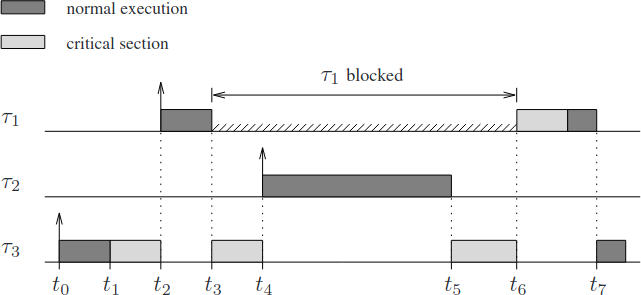
\includegraphics[width=0.6\textwidth]{media/image50.png}
    \caption{Esempio di Priority Inversion}
\end{figure}

Nell'esempio, $\tau_1$ è il task a priorità massima e viene bloccato da $\tau_3$ perché utilizza prima la risorsa critica.

\section{Gestione delle risorse in RTOS}

Il problema dello scheduling con vincoli su risorse è strettamente legato a quello dei sistemi operativi real-time. In particolare, bisogna tenere conto dei tempi di bloccaggio per il test di schedulabilità.

\textbf{Terminologia}:
\begin{itemize}
    \item $B_i$: massimo tempo per cui $\tau_i$ risulta bloccato.
    \item $z_{i,k}$: una sezione critica per $\tau_i$ dal semaforo $S_k$.
    \item $\delta_{i,k}$: durata della sezione critica più lunga $Z_{i,k}$.
    \item $\sigma_i$: insieme di semafori utilizzati da $\tau_i$.
    \item $\gamma_{i,j}$: insieme delle più lunghe sezioni critiche che possono bloccare $\tau_i$ accedute dai task $\tau_j$ ($j > i$).
\end{itemize}

\section{Protocolli di Accesso alle Risorse}

Per risolvere la priority inversion, si utilizzano protocolli specifici:

\subsection{Non-Preemptive Protocol (NPP)}

Si tratta di un protocollo molto semplice che assicura al processo che accede alla sezione critica la possibilità di eseguire senza interruzioni, eliminando di fatto la prelazione. Ciò avviene assegnando al processo $\tau_i$ la priorità più alta di tutti gli altri task nel sistema: $p_i(R_k) = \max_h(P_h)$.

Pur essendo di semplice implementazione, è altamente inefficiente in quanto blocca anche i task che non utilizzano la risorsa condivisa.

\subsection{Highest Locker Priority (HLP)}

È un protocollo molto simile al non preemptive. Modifica le priorità solo ai task che devono usare la sezione critica. Un processo $\tau_i$ che utilizza una risorsa $R_k$ ha una priorità dinamica \[p_i(R_k) = \max_h(P_h | \tau_h \text{ usa } R_k)\].
Questo valore è detto \textbf{priority ceiling} della risorsa: $C(R_k)$. Per questo motivo il protocollo è anche detto \textbf{Immediate Priority Ceiling}.

Anche con questo protocollo si verificano attese inutili in quanto un processo può non usare sempre la risorsa critica.
Nel calcolo delle priorità dinamiche, verrà fatta sempre una stima pessimistica ignorando se il processo per quell’istanza effettui o meno la preemption.

\subsection{Priority Inheritance Protocol (PI)}

Si tratta di uno dei protocolli più utilizzati nei sistemi real-time perché offre la possibilità di fare analisi di schedulabilità. Quando un task $\tau_i$ risulta bloccato su un semaforo, trasmette la sua priorità a $\tau_j$ che detiene il semaforo. Quindi $\tau_j$ riprende l'esecuzione con $p_j = p_i$. Si dice che $\tau_j$ eredita la priorità di $\tau_i$. Priority inheritance tuttavia non risolve il problema dell'attesa circolare e deadlock.

I passi del protocollo sono:
\begin{itemize}
    \item Task sono schedulati in base alle loro active priority. Task con la stessa priorità sono eseguiti con FCFS;
    \item Quando un task $\tau_i$ prova ad entrare in una regione critica $z_{i,k}$ per la risorsa $R_k$ che è occupata già da un task $\tau_j$ con $j > i \to p_j < p_i$, si dice che $\tau_i$ è bloccato da $\tau_j$ che detiene la risorsa. Altrimenti $\tau_i$ entra nella sezione critica;
    \item Quando un task $\tau_i$ risulta bloccato su un semaforo, trasmette la sua priorità a $\tau_j$ che detiene il semaforo. Quindi $\tau_j$ riprende l'esecuzione con $p_j = p_i$. Si dice che $\tau_j$ eredita la priorità di $\tau_i$;
    \item Quando $\tau_j$ esce da una sezione critica, sblocca il semaforo insieme al task a più alta priorità bloccato su quel semaforo.
        \begin{itemize}
            \item La priorità di $\tau_j$ viene ripristinata a $P_j$ se non c'è nessun altro task bloccato sulla risorsa $R_k$;
            \item Altrimenti prende la massima priorità del task bloccato su $R_k$
        \end{itemize}
    \item L'eredità della priorità è transitiva. Se $\tau_3$ blocca $\tau_2$ e $\tau_2$ blocca $\tau_1$ allora $\tau_3$ eredità la priorità di $\tau_1$ attraverso $\tau_2$;
\end{itemize}

In generale, la priorità $p_j(R_k)$ è:

\[ p_j(R_k) = \max\{P_j, \max_h\{P_h | \tau_h\; bloccato\; su\; R_k\}\}\]

Questo protocollo comporta due Tipi di bloccaggio:
\begin{itemize}
    \item \textbf{Bloccaggio diretto (direct blocking)}: avviene quando un processo $J_H$ con priorità nominale superiore a quella del task che ha ereditato la priorità viene bloccato a causa della nuova priorità ereditata.
    \item \textbf{Bloccaggio indiretto (push-through blocking)}: un processo a priorità intermedia $J_M$ resta bloccato da un processo $J_L$ a priorità inferiore che ha ereditato la priorità di $J_H$.
\end{itemize}

\paragraph{Analisi di schedulabilità}
Con PI è possibile calcolare un upper-bound per la schedulabilità del task set.
Assumendo RM, deve essere:

\begin{equation}
    \forall i = 1...n \sum_{k=1}^i\frac{C_k}{T_k} + \frac{B_i}{T_i} \leq i(2^{(1/i)} - 1)
\end{equation}
Inoltre, con DM è possbiile effettuare la RTA aggiungendo al tempo di risposta quello di bloccaggio.

\begin{equation}
    R_i = C_i + B_i + \sum_{k=1}^i\lceil\frac{R_i}{T_k}\rceil C_k
\end{equation}

a come si calcola il tempo di bloccaggio? Sia $\delta$ la matrice dei tempi di bloccaggio delle massime durate delle sezioni critiche. Sia $c(R_k)$ il ceiling della risorsa $c(R_k) = \max_j{P_j : \tau_j\; usa\; R_k}$. Il tempo di bloccaggio è:

\begin{equation}
    B_i = \min{B_i^l, B_i^s}
\end{equation}

con:
\begin{equation}
    B_i^l =\sum_{i+1}^n \max_k\{\delta_j,k: C(S_k) \geq P_i\}
\end{equation}

e:
\begin{equation}
    B_i^s =\sum_{k}^m \max_{j>i}\{\delta_j,k: C(S_k) \geq P_i\}
\end{equation}

\paragraph{Esempio}
Nell'esempio si riporta il calcolo del tempo di bloccaggio data la seguente matrice:

\begin{center}
\renewcommand{\arraystretch}{1.3}
\begin{tabular}{|c|c|c|c|}
\hline
 & $\boldsymbol{C_i}$ & $\boldsymbol{T_i}$ & $\boldsymbol{B_i}$ \\ \hline
$\boldsymbol{\tau_1}$ & 3 & 10 & 5 \\ \hline
$\boldsymbol{\tau_2}$ & 4 & 20 & 6 \\ \hline
$\boldsymbol{\tau_3}$ & 6 & 30 & 0 \\ \hline
\end{tabular}
\end{center}

\begin{itemize}
    \item Il test richiede tre passi, per $i$ da 1 a 3:
    \begin{enumerate}
        \item $C_1/T_1 + B_1/T_1 = 0.8 \le 1$
        \item $C_1/T_1 + C_2/T_2 + B_2/T_2 = 0.8 \le 0.83$
        \item $C_1/T_1 + C_2/T_2 + C_3/T_3 = 0.7 \le 0.78$
    \end{enumerate}
\end{itemize}

Per calcolare $B_i^l$ si prendono tutti i task $\tau_j$ con $j > i$:
\begin{itemize}
    \item Per ogni $\tau_i$ si identificano l'insieme delle sezioni critiche che possono bloccare $\tau_j$;
    \item Per ogni insieme identificato, relativo ai processi $\tau_j$, identifichiamo la sezione critica a durata massima $Z_{j,k}$ e sommiamo la loro durata $\delta_{i,k}$. Si ottiene $B_i^l$.
\end{itemize}

Per calcolare $B_i^s$ si prendono tutti i semafori $S_k$ con $1 \le k \le m$:
\begin{itemize}
    \item Per ogni semaforo si individua l'insieme delle sezioni critiche da esso gestite che possono bloccare $\tau_i$: $\gamma_{i,k}$.
    \item Per ogni insieme $\gamma_{i,k}$ si individua la sezione critica di massima durata e le si somma tra loro, si ottiene $B_i^s$.
\end{itemize}

$\begin{aligned}
&B_1^l = 8 + 7 + 5 = 20 \\
&B_1^s = 7 + 8 = 15
\end{aligned} \implies B_1 = 15$

$\begin{aligned}
&B_2^l = 7 + 5 = 12 \\
&B_2^s = 7 + 6 + 3 = 16
\end{aligned} \implies B_2 = 12$

$\begin{aligned}
&B_3^l = 5 \\
&B_3^s = 5 + 4 + 3 = 12
\end{aligned} \implies B_3 = 5$

$B_4^l = B_4^s = 0 \implies B_4 = 0$

\subsection{Priority Ceiling Protocol (PC)}

Questo protocollo estende priority inheritance con un controllo che consente di evitare il problema delle attese circolari e deadlock. Non consente a un task di accedere ad una sezione critica se ci sono semafori bloccati che possono bloccarlo. Una volta che un task entra nella sua prima sezione critica non può mai essere bloccato da uno a priorità più bassa.

\begin{itemize}
    \item Ogni semaforo $S_k$ ha assegnato un livello di priorità (detto priority ceiling) $C(S_k)$ pari al livello di priorità più alto tra i task che possono bloccarlo. È un valore statico che può essere calcolato off-line;
    \item Sia $\tau_i$ il task a più alta priorità che viene assegnato al processore. Per entrare in una sezione critica gestita da $S^*$, deve essere $\tau_i$ deve avere un priorità più alta di $C(S^*)$. Se $P_i \leq  C(S^*)$, allora l'accesso alla sezione viene negato e si dice che $\tau_i$ i è bloccato sul semaforo $S^*$ dal task che detiene il lock su $S^*$.
    \item Quando $\tau_i$ è bloccato su un semaforo, esso trasmette la priorità al task. $\tau_j$ che detiene il semaforo. Quindi analogamente a PI, il task $\tau_j$ eseguirà per il resto della sezione critica con $p_i$
    \item Quando $\tau_j$ esce dalla sezione critica, sblocca il semaforo e il task a più alta priorità bloccato sul semaforo. La priorità di $\tau_j$ diventa $P_j$ se non ci sono altri task bloccati da $\tau_j$. Altrimenti viene messa pari alla più alta priorità sul task bloccato da $\tau$
    \item La priorità può essere ereditata per via transitiva.
\end{itemize}


\chapter{Virtualizzazione}

La virtualizzazione è una tecnica utilizzata per condividere la stessa piattaforma tra sistemi operativi diversi. Un sistema virtualizzato si dice che ospita delle \textbf{macchine virtuali} (VM), gestite da un \textbf{Virtual Machine Monitor (VMM)} o \textbf{hypervisor}.

In generale, ciò porta diversi benefit quali:
\begin{itemize}
    \item \textbf{safety e security}: guasti e bug su una VM non impattano le altre (\textbf{sandboxing}).
    \item \textbf{coesistenza}: diversi sistemi operativi sulla stessa piattaforma (es. sistemi legacy).
    \item \textbf{motivi economici}: riduzione dei costi hardware e di gestione.
    \item \textbf{load balancing}: facilità nel migrare processi o replicare stack applicativi.
    \item \textbf{developer experience}: è molto più facile testare un'applicazione sotto diversi sistemi operativi;
\end{itemize}

Esistono due tipi di hyperrvisor:
\begin{enumerate}
    \item \textbf{Tipo 1 (Bare Metal)}: funziona a diretto contatto con l'hardware (es. Xen, VMware ESXi).
    \item \textbf{Tipo 2 (Hosted)}: funziona al di sopra di un sistema operativo host (es. VirtualBox, KVM).
\end{enumerate}

Il problema principale è che le VM credono di essere l'elemento più privilegiato. Un SO ha una parte \textbf{kernel mode} (privilegiata) e una \textbf{user mode}. Il VMM deve intervenire per rendere possibile la coesistenza di diversi kernel.

\section{Tecniche di Virtualizzazione}

Dal punto di vista formale, Popek e Goldeberg enunciarono i requisiti principali per supportare la virtualizzazione. Innanzitutto, viene fatta una distinzioni tra le istruzioni di una CPU: non tutte sono uguali e su alcune di queste deve agire l'hypervisor. In particolare, le \textbf{sensitive instructions} indicano istruzioni per accedere all'I/O, impostazioni dell'MMU e tutte le altre che devono essere eseguite in kernel mode e non è possibile eseguire in user mode. Le \textbf{privileged instructions} sono quelle istruzioni che se eseguite in modalità utente (e devono essere in modalità kernel) generano una trap. Nell'articolo, Popek e Goldeberg mostrano che una macchina è virtualizzabile solo se le sensitive instructions sono un sottoinsieme di quelle privileged. Questo articolo dimostra anche che la prima architettura x86 non è fatta per essere virtualizzata. Infatti, molte sensitive instructions non eseguivano trap. Ad esempio, l'accesso a registro di stato da parte di un processo utente si traduceva semplicemente in una no-op. Il supporto hardware alla virtualizzazione detta VT per Intel e SVM per AMD fu introdotto a partire dal 2005.

Le principali tecniche di virtualizzazione sono:
\begin{itemize}
    \item \textbf{Full virtualization}: la macchina virtuale guest non sa di essere virtualizzata. Può essere realizzata o con la binary translation o con la trap and emulate.
    \item \textbf{Para-virtualizzazione}: la macchina virtuale guest sa di essere virtualizzata, quindi modifica alcuni driver o parti del suo codice per funzionare meglio con l'hypervisor. Può essere realizzato con un'interfaccia software dell'hypervisor (API) in cui vengono esposte delle funzioni Hypercall.
\end{itemize}

\subsection{Trap and Emulate}

È una tecnica utilizzata dagli hypervisor per eseguire le sensitve instructions (secondo Goldberg e Popek queste istruzioni devono effettuare trap). In pratica, quando il guest OS esegue un'istruzione sensitiva questa viene intercettata (attraverso la trap) dal VMM ed emulata per far coesistere diverse macchine virtuali.

\subsection{Ring deprivileging}

L'architettura x86 ha 4 livelli di protezione (\textbf{rings}). In un sistema non virtualizzato, il kernel è in ring 0 e le app in ring 3.
\begin{itemize}
    \item \textbf{Modello 0/1/3}: l'hypervisor è in ring 0, il kernel guest in ring 1 e le app in ring 3.
    \item \textbf{Modello 0/3/3}: sia kernel guest che app sono in ring 3 (usato per hypervisor di tipo 2).
\end{itemize}

Senza supporto hardware, vengono usati sia la binary translation che i protection ring. L'architettura x86 ha 4 protection mode. In un sistema non virtualizzato, il ring 0 viene dato al kernel e i processi utente vengono eseguiti in in ring 3. Parlando di hypervisor bare metal, le macchine virtuali usavano il ring 1, mentre quello 0 viene assegnato all'hypervisor (modello 0/1/3).

\subsection{Binary Translation}

Consiste nel tradurre \textbf{basic blocks} di codice in istruzioni compatibili. Prima dell'esecuzione, il VMM esamina il codice e rimpiazza le istruzioni sensitive con chiamate alle procedure dell'hypervisor. Questa tecnica è così semplice e si presta bene alle ottimizzazioni. Ad esempio, se un blocco tradotto termina, o viene concatenato con un'altra istruzione sensitiva, si può evitare di dare il controllo all'hypervisor. Inoltre, in alcune implementazioni si preferisce usare questa approccio anche per le parti che dovrebbero eseguire in trap and emulate perché le trap invalidano le cache e, in generale, hanno performance peggiori della traduzione dei blocchi. In generale, queste considerazioni hanno senso anche in hypervisor di tipo 2. Il controllo hardware viene effettuato attraverso moduli kernel che comunicano con il sistema operativo host. Un modello simile a quello mostrato è quello in cui viene utilizzato il livello di privilegio 3 sia per i kernel delle macchine virtuali sia per i guest; mentre il VMM esegue a ring 0 (modello 0/3/3). La virtualizzazione con ring deprivileging ha molti problemi che non possono essere risolti via software senza impattare di molto le performance dei guest o violando i principi di fidelity di un VMM. Alcuni di questi problemi:
\begin{itemize}
    \item \textbf{Ring aliasing}: quando un'istruzione viene eseguita ad un ring diverso da quella per cui è stata pensata. Un guest OS può semplicemente ispezionare dei registri per capire che non sta eseguendo con privilegio 0.
    \item \textbf{Address-space compression}: i sistemi operativi si aspettano di poter operare su tutto lo spazio di indirizzamento virtuale, ma ciò non è possibile. Il VMM ha bisogno di un suo spazio di indirizzamento e deve anche prendere un po' di memoria dai guest perché ha bisogno di allocare codice e strutture dati per gestire i cambi di contesto. Quindi bisogna prevenire che i guest entrino in queste aree di memoria protette.
    \item \textbf{Non faulting access to privileged state}: alcune istruzioni possono eseguire anche in modalità utente e possono accedere a strutture dati critiche a ring 0. L'accesso a queste strutture come il registro PTA (che contiene l'indirizzo della Virtual Hash Page Table (VHPT)) può far capire al guest di non essere da solo nel sistema e non avere il pieno controllo della CPU.
    \item \textbf{Adverse impacts on guest transitions}: non è possibile utilizzare le istruzioni SYSENTER e SYSEXIT per avere system call a bassa latenza. Queste istruzioni portano sempre ad eseguire in ring 0 che non corrisponde alla modalità corretta per i guest. Un guest che usa SYSENTER non va in kernel mode, ma nel VMM. Il VMM deve poter emulare queste due istruzioni. Inoltre, l'architettura Intel supporta interruzioni veloci che non mettono dati in memoria, ma passano informazioni sull'interruzione in registri del processore. Tutti gli interrupt handler usano questi registri. Nel caso virtualizzato si genererebbero molte trap che devono essere intercettate e gestite dal VMM.
    \item \textbf{Ring compression} per proteggere il VMM bisogna usare un meccanismo di protezione della memoria: paging. Per come è fatta, la tabella delle pagine in IA--32 non distingue i livelli di privilegio tra 0 - 2. Questo vuol dire che il guest OS deve eseguire a livello 3 per non impattare il VMM.
    \item \textbf{Access to hidden state}: alcuni registri del processore non possono essere acceduti via software. Quindi ci potrebbero essere problemi di sicurezza tra guest. Il VMM non è in grado di ripristinare questi registri.
\end{itemize}

\section{Supporto Hardware: Intel VT-x}

Introduce due modalità: \textbf{VMX root} (per il VMM) e \textbf{VMX non-root} (per i guest). Entrambe hanno i 4 ring. Il passaggio avviene tramite \textbf{VM entry} e \textbf{VM exit}. VTx introduce la struttura \textbf{VMCS (Virtual Machine Control Structure)} per gestire lo stato di guest e host.

\section{Virtualizzazione della Memoria}

Il VMM deve gestire l'allocazione fisica per ogni guest.
\begin{itemize}
    \item \textbf{Shadow page tables}: il VMM tiene traccia delle tabelle del guest in software. Ogni modifica causa un \textbf{hypervisor-induced page fault}.
    \item \textbf{Supporto Hardware (EPT - Extended Page Tables)}: rimuove le trap per accedere alla memoria distinguendo tra \textbf{guest physical addresses} e \textbf{host physical addresses}.
\end{itemize}

\section{Virtualizzazione I/O}

\begin{itemize}
    \item \textbf{Trap and emulate}: il VMM intercetta gli accessi ai registri dei dispositivi.
    \item \textbf{Device pass-through}: consente a una VM di usare direttamente l'indirizzo fisico del dispositivo (tramite \textbf{I/O MMU}).
    \item \textbf{Paravirtualizzazione}: VM e VMM comunicano tramite \textbf{shared memory} e \textbf{hypercall}.
    \item \textbf{SR-IOV (Single root I/O virtualization)}: bypassa l'hypervisor configurando istanze indipendenti (\textbf{Virtual Functions}) per i dispositivi.
\end{itemize}


\chapter{Mixed Criticality Systems}

La rapida evoluzione tecnologica ha portato alla necessità di far coesistere applicazioni con diversi gradi di criticità sullo stesso hardware (es. ECU automotive che gestiscono sia controlli di guida che infotainment). La sfida è conciliare i requisiti di \textbf{safety} (isolamento) con quelli di \textbf{efficienza} (condivisione delle risorse).

\section{Modello di Vestal}

Il primo modello per i sistemi a criticità mista è quello di \textbf{Vestal}. Il sistema prevede diversi livelli di criticità $L_i$ e ogni task è caratterizzato da parametri che dipendono da $L_i$:
\begin{itemize}
    \item $C_i(L)$: WCET per ogni livello di criticità. Vale $C_i(l) \le C_i(l+1)$.
    \item $D_i$: deadline relativa.
    \item $T_i$: periodo del task.
    \item $L_i$: criticità del task.
\end{itemize}

Dato $L_i > L_j$, per assicurare vincoli più stringenti per i task hard real-time si fanno stime più conservative: $T(L_i) \le T(L_j)$ e $C(L_i) \le C(L_j)$.
Un sistema a due livelli viene detto \textbf{dual-criticality} (\textbf{HI} e \textbf{LO}).

\subsection{Livelli di integrità e modi di funzionamento}

Il sistema può evolvere a partire dalla modalità a criticità minima. Gli eventi cruciali sono i \textbf{cambi di modalità}: se un task esegue oltre il suo $C_i$ (overrun), si verifica un cambio di modalità verso un livello di criticità superiore. In modalità ad alta criticità, i task a bassa criticità possono essere sospesi o degradati per garantire le deadline dei task critici.

\subsection{Limiti del modello di Vestal}

Crea un forte accoppiamento tra applicazioni e grado di criticità. Secondo questo modello, ogni applicazione (anche se non richiesto) deve essere certificata con il SIL massimo, comportando costi di certificazione esorbitanti.

\section{Scheduling con Deadline Monotonic}

Al modello di Vestal è stata applicata la RTA iterativa:
\[ R_i^{(k+1)} = \sum_{j:p_j \le p_i} \left\lceil \frac{R_i^{(k)}}{T_j} \right\rceil C_{j, L_i} \]
Somma i contributi dei task a priorità più alta nel livello di criticità $L_i$ corrente. Tuttavia, DM non è ottimo nel caso multi-criticality.

\subsection{Run-time slicing (Period transformation)}
Il run-time slicing o (period transformation) è una tecnica che serve a rendere schedulabile l'insieme nell'esempio
precedente risolvendo il problema di deadline monotonic. Infatti, preso una situazione simile, un task a priorità più alta con livello di integrità superiore, ma con periodo maggiore può essere fatto eseguire prima.
Run time slicing prevede di dividere il periodo del task $\tau_i$ $T_j$ di un fattore $n$ ottenendo così:

\[T_j'=\frac{T_j}{n}\]

Dove $n$, è una costante intera che serve a ridurre il periodo di quanto basta per consentirne l'esecuzione. La tecnica
prevede anche la riduzione del tempo di calcolo di $C_j$ (in base al livello Li corrente) secondo la stessa relazione:

\[C_j'=\frac{C_j}{n}\]

Questo vuol dire che l'ultimo job può finire di eseguire prima poiché la divisione è sempre a resto nullo. Quindi,
applicando la formula al RTA si ottiene:

\[ R_i^{k+1} = \sum_{j:p_j\leq p_i}\lceil\frac{R_i^k}{T_j/n}\rceil C_{j,L_i} = \sum_{j:p_j\leq p_i}n\lfloor\frac{R_i^k}{T_j}\rfloor C_{j,L_i}\]

\subsection{Assegnazione delle priorità di Audsley}
Questa tecnica proposta da Audsley è ottima e si basa su due lemmi:

\begin{enumerate}
    \item  il WCET di un task $\tau_i$ può essere determinato (attravero la RTA) conoscendo solamente tutti i task priorità maggiore di $\tau_i$ ma senza conoscere la regola specifica con cui si assegneno le priorità;
    \item Se un task è schedulabile con una certa priorità assegnata, esso rimarrà schedulabile se la sua priorità aumenta (se le altre priorità restano invariate)
\end{enumerate}

L'algoritmo inizia senza che un'attività abbia una priorità assegnata. Le priorità sono assegnate dal più basso, in modo che la prima attività sarà quella con la priorità più bassa. Ad ogni passaggio, viene selezionata un'attività tra quelle ancora a cui manca un task prioritario e viene assegnato la successiva priorità. L'attività selezionata in ogni passaggio è qualsiasi tra quelli che saranno schedulabili se assegnato alla prossima priorità più alta. Con il lemma 1, questo può essere determinato senza conoscere le priorità esatte che vengono assegnate ai task, ma solo che quelli rimanenti riceveranno una priorità più alta.

L'algoritmo termina senza successo in qualsiasi fase in cui nessuna delle attività rimanenti è schedulabile, o con
successo quando tutte le attività sono state assegnate a priorità.
Lemma 2 ci assicura che l'algoritmo troverà un'assegnazione prioritaria fattibile se esiste.

\section{Scheduling gerarchico}
Il modello di Vestal è stato il primo approccio con risultati concreti per i sistemi a criticità mista, ma come visto ha molte limitazioni. Un approccio con una migliore separazione è lo scheduling gerarchico. Nello scheduling gerarchico si fa riferimento ad applicazioni a cui viene assegnato un budget che vengono schedulati su un primo livello di piattaforma e ai thread all'interno di esse. Esistono due grandi famiglie di scheduling gerarchico:

\begin{itemize}
    \item globale: si decide quale applicazione $A_k$ debba eseguire;
    \item locale: si decide quale task $\tau_{i,k}$ dell'applicazione $A_k$ debba eseguire;
\end{itemize}

Analizziamo 3 approcci per lo scheduling gerarchico:
\begin{itemize}
    \item Architettura Open System;
    \item FTP gerarchico;
    \item H-CBS
\end{itemize}

\subsection{Architettura Open System}


\end{document}
